%
% *** SECTION 5 ***
%

As discussed in \S 2.2.3 of SDT15 (written by members of our team), the
HLS Imaging survey will (in its current design) measure the shapes of
nearly 400 million galaxies in 3 near-infrared (NIR) bands, plus fluxes in a 4th band
to improve photometric redshifts (photo-$z$).  With a data set two orders-of-magnitude
larger than the current state of the art \cite{2012MNRAS.427..146H,Becker2015},
the WFIRST weak lensing program will
measure the cosmic expansion history and the growth of structure with
exquisite statistical precision, demanding corresponding advances in the
control of WL systematics.  The cosmic shear power spectrum, which is the
basic WL observable, depends on both the distance-redshift relation $D(z)$
and the power spectrum of matter clustering $(\Omega_m h^2)^2 P_m(k,z)$.
The WL survey will also enable high-precision cosmological constraints
from galaxy-galaxy lensing (GGL) and from galaxy clusters, which can be
identified in either the HLS or external data sets and characterized with
the help of WFIRST WL.  The \CoLi\ forecasting tool can predict the constraints
from these methods individually and in combination with complementary
probes such as BAO, RSD, supernovae, and the CMB.
While all aspects of our investigation are interconnected, we
separate the discussion into more tightly connected loops: requirements,
image simulations, and algorithm development at level of pixels and shape measurement;
issues related to photometric calibration and photometric redshifts;
development of methods for cosmological analysis of WFIRST
data and testing them on simulated data; and finally methods for
systematic error testing and mitigation.

\subsection{Requirements (D1, D3, D4, D5)}
\label{sec:wl_requirements}
%================================================
\Auth{Chris, Rachel M, Mike}

The definition of WFIRST requirements will
%proceed through a phased approach with several
%stages of increasing detail and maturity,
start in pre-Phase A and continue through
CDR. In the early stages, we will focus on identifying the driving requirements for the
mission (e.g., those related to total throughput, wavefront error and wavefront stability,
and any calibration requirements that would require dedicated hardware or special operational modes).
Simple simulation tools will be used for this stage, where fast turnaround times and
conservative assumptions will be prioritized over the true end-to-end simulations that
will be required for the analysis. As the project matures, we will consider the more
complete list of requirements (e.g., specifications on data products)
and work with the WFIRST Science Centers (WSC) to build the fully
realistic simulations needed to test reduction and analysis pipelines.

Our existing tools (the ETC, operations simulations, and \CoLi)
allow us to forecast the statistical power of the WL survey for a specified
observing strategy and time allocation and to evaluate the impact of
hardware or strategy changes on cosmological constraints (see \S 6.2).
The challenge for the SIT is to define requirements that ensure control
of systematic uncertainties at the level of these statistical errors.
WL systematics fall into two broad categories, instrumental/algorithmic
effects tied directly to the measurements and astrophysical effects
tied to the cosmological interpretation of the measurements.  The former
affect engineering requirements, while the latter must be predicted
theoretically or constrained through observations.

Our basic strategy for defining instrumental/algorithmic requirements
is to create simulated HLS images with varying levels of realism, analyze
them with proto-type data reduction and WL pipelines, and compare the
resulting measurements to the simulation inputs. We will determine
the sensitivity of WL shear measurements to each effect,
and then flow down requirements from nuisance parameters in
\CoLi\ (e.g., spurious shear) to hardware requirements that can be compared to integrated
modeling results (e.g., wavefront stability).
Our simulation
framework will build on the public code {\tt GalSim} \cite{2015A&C....10..121R}, which already
includes a WFIRST-AFTA module and
to which Co-Is Jarvis and Mandelbaum are lead contributors.  Our proto-type pipelines will
build on codes for image analysis and shear measurements developed
over many years by Co-Is Hirata, Jarvis, Lupton, and Mandelbaum
and their collaborators for analysis of SDSS, DES, HSC, and LSST imaging
\cite{Lupton2001, 2003MNRAS.343..459H, 2005MNRAS.361.1287M,
2012MNRAS.420.1518M, 2011arXiv1111.6958H, Jarvis2015}.
WL algorithms are an active area of research,
and we will integrate promising new approaches as our investigation
progresses.  Our overall framework is analogous to, but more %tightly
focused than, the GREAT3 challenge led by Mandelbaum \cite{2014ApJS..212....5M},
including the use of different simulation branches where effects are turned on and off
(separately or together) to probe the %origins of any
biases %or unexpected behaviors
resulting from individual or combined effects.
%we will draw on lessons learned from this effort and its predecessors.

In the domain of instrument- and pipeline-related systematic errors,
each error must be evaluated according to the following criteria:
(i) What is the raw magnitude of the systematic error compared to statistical errors?
(ii) What is the approach to modeling and removing that systematic error? What cross-checks will be necessary to
validate that this has been done correctly? (iii) Are there
implications to the optimal observing strategy (e.g., dithering, repeat observations, dedicated calibration
observations)? (iv) Are there implications for the hardware requirements (e.g.,
stability, pre-flight characterization, or dedicated flight calibration hardware)?

As an example: optical aberrations induce PSF ellipticity that is 2 orders of magnitude
greater than WFIRST weak lensing requirements if uncorrected. It is not practical to
eliminate the effect in hardware by requiring the wavefront to be perfect at the few nm
level in a wide-field instrument, so a model of the PSF will have to be built.
Some contributions to the PSF (e.g., jitter and guiding errors) will need to be measured separately for each
exposure. Others vary on longer time scales (e.g., due to thermal changes in the optics)
and imply a trade-off between stability requirements
and the noise on a measurement of the relevant parameter from a set of $N$ exposures.
We will use these considerations to turn high-level requirements on knowledge of the PSF into
lower-level requirements on thermal stability and on the operations plan.

Detector systematics are special because their absolute amplitudes may be difficult for the vendor to control or even test.
We thus anticipate absolute
requirements only on the largest systematic effects such as inter-pixel capacitance (IPC) and persistence, which are
being addressed as part of the technology development program. There will be many subtler
effects arising in the detectors
(examples might include NIR-detector analogues of the brighter-fatter effect,
color-dependent charge diffusion, etc.); we will set requirements on the knowledge of these.
We will pay special attention to methods of measuring these effects on-orbit using a combination of
ground characterization, dedicated calibration modes, and the survey data itself,
and the interaction with survey operations and stability requirements (on e.g., focal plane temperature).
We will coordinate the best approach to these effects with the Project
and with collaborators Seiffert and Shapiro.  Shapiro leads the
Precision Projector Laboratory (PPL), a JPL facility designed to
emulate WFIRST weak lensing data using scenes focused onto WFIRST
NIR-detectors.  Systematics identified thusly will be studied and
mitigated in collaboration with the SIT.  Co-I Hirata advises the PPL on
image analysis software and interpretation of results \cite{Rowe:2011wj, Seshadri:2013xla}.

%We will treat astrophysical systematic errors differently because one cannot write
%a requirement on e.g., the behavior of a galaxy, so the requirements are instead on the
%algorithmic strategies for mitigating the systematic errors.
%A typical mitigation strategy for intrinsic alignments (IA) of galaxy shapes would involve
%jointly modeling the effects of IA on the
%tomographic two-point functions of the shear and the galaxies.
%As shown by, e.g.,
%\cite{2007NJPh....9..444B}, the need to marginalize over IA results in
%more stringent requirements on how well the photometric redshift error distributions are
%known.
%In some cases, the effects of astrophysical uncertainties are degenerate with measurement
%uncertainties; for instance the effect of baryonic physics on the lensing power spectrum
%is partially degenerate with photometric redshift errors \citep{2012JCAP...04..034H}.
%As we cannot place a requirement on baryonic physics, this can result in
%more stringent requirements for the effects we can control, such as photometric redshifts.

Cluster cosmology is generally considered to be less demanding in terms of hardware requirements than
cosmic shear, since the large galaxy over-densities and shear signals are not as easily masked by
subtle optical aberrations or detector behaviors. Nevertheless, it may place new requirements
on survey footprint/operations (to ensure overlap with other data sets); pipeline behavior in
crowded fields (e.g., \cite{2015MNRAS.449.1259S}); and ancillary data products and simulations to describe, e.g., changes in selection
effects and source redshift distributions in the presence of blending and magnification.
WL requirements lead Hirata will work closely with cluster lead Weinberg to ensure that these
requirements are captured in the flow-down.

% -- notes from DHW --
%
%\bi
%\item  Dark energy requirements for HLS Imaging and associated
% instrument requirements, at level of image sampling,
% PSF stability, software performance, etc.
%\item  Simulations at level of frames, focal plane.  Data challenges.
%\item  Proto-type pipelines that either meet requirements or inform
% what is needed to meet them.  Assessment of photometry errors,
% shape measurement errors.
%\ei
%
%DW comments on this subsection: Idea of proto-type pipelines is that
%they are capable of analyzing the same data sets that our simulations
%are producing.  They are used to test algorithm development, test the
%impact of sampling, PSF uncertainty, etc., and provide an existence
%proof of meeting requirements or an identification of what challenges
%remain to be solved.  Not intended to be a full up pipeline that
%deals with the data flow from WFIRST.  However, will work closely
%with Project so that proto-types we develop can be ingested and that
%we take advantage of work being done by the project.

\textbf{Below is some new text from Rachel M.  It needs to be put in the right place.  If more
information or detail is needed, please let me know.}

\subsubsection{Polarization effects}
During early 2017, work was carried out to assess the approximate level of an effect that could
cause weak lensing systematics, but that had never been previously considered by the weak lensing
community.  This effect is polarization-dependent quantum efficiency (due to e.g.\ different
reflectivity of various coatings for different polarizations of light).  Since the light from
edge-on disk galaxies typically has some low level polarization perpendicular to the disk, any
polarization-dependence of the QE could result in a preferential selection of such galaxies based on
their orientation in the focal plane.  This would violate the baseline assumption in a weak lensing
analysis, which is that all coherent galaxy alignments are due to gravitational lensing.

A student at CMU, Brent Tan, worked with Rachel Mandelbaum and Chris Hirata on a simple toy model
for this effect.  The toy model had two parameters: the fraction of the disk galaxy light that is
polarized, and the relative attenuation of that perpendicular polarization component (both numbers
in the range $[0,1]$).  For each point in that parameter space, the coherent shear due to selection
bias was calculated; see results in Figure~\ref{fig:polarization}.  Finally, the results were
modified to account for the fact that not all disk galaxies are viewed edge-on and that not all
galaxies are disks, giving a net coherent shear due to this selection bias of $\sim 3\times
10^{-4}$.  The results are still quite uncertain because our fiducial values for the disk
polarization fraction were based on observations of nearby galaxies, not $z\sim 1$ disks.  However,
this is large enough to be relevant for WFIRST, so this systematic needs to be evaluated more
carefully and requirements placed in future.  A publication on this topic will be prepared during
summer 2017.
\begin{figure}
\begin{center}
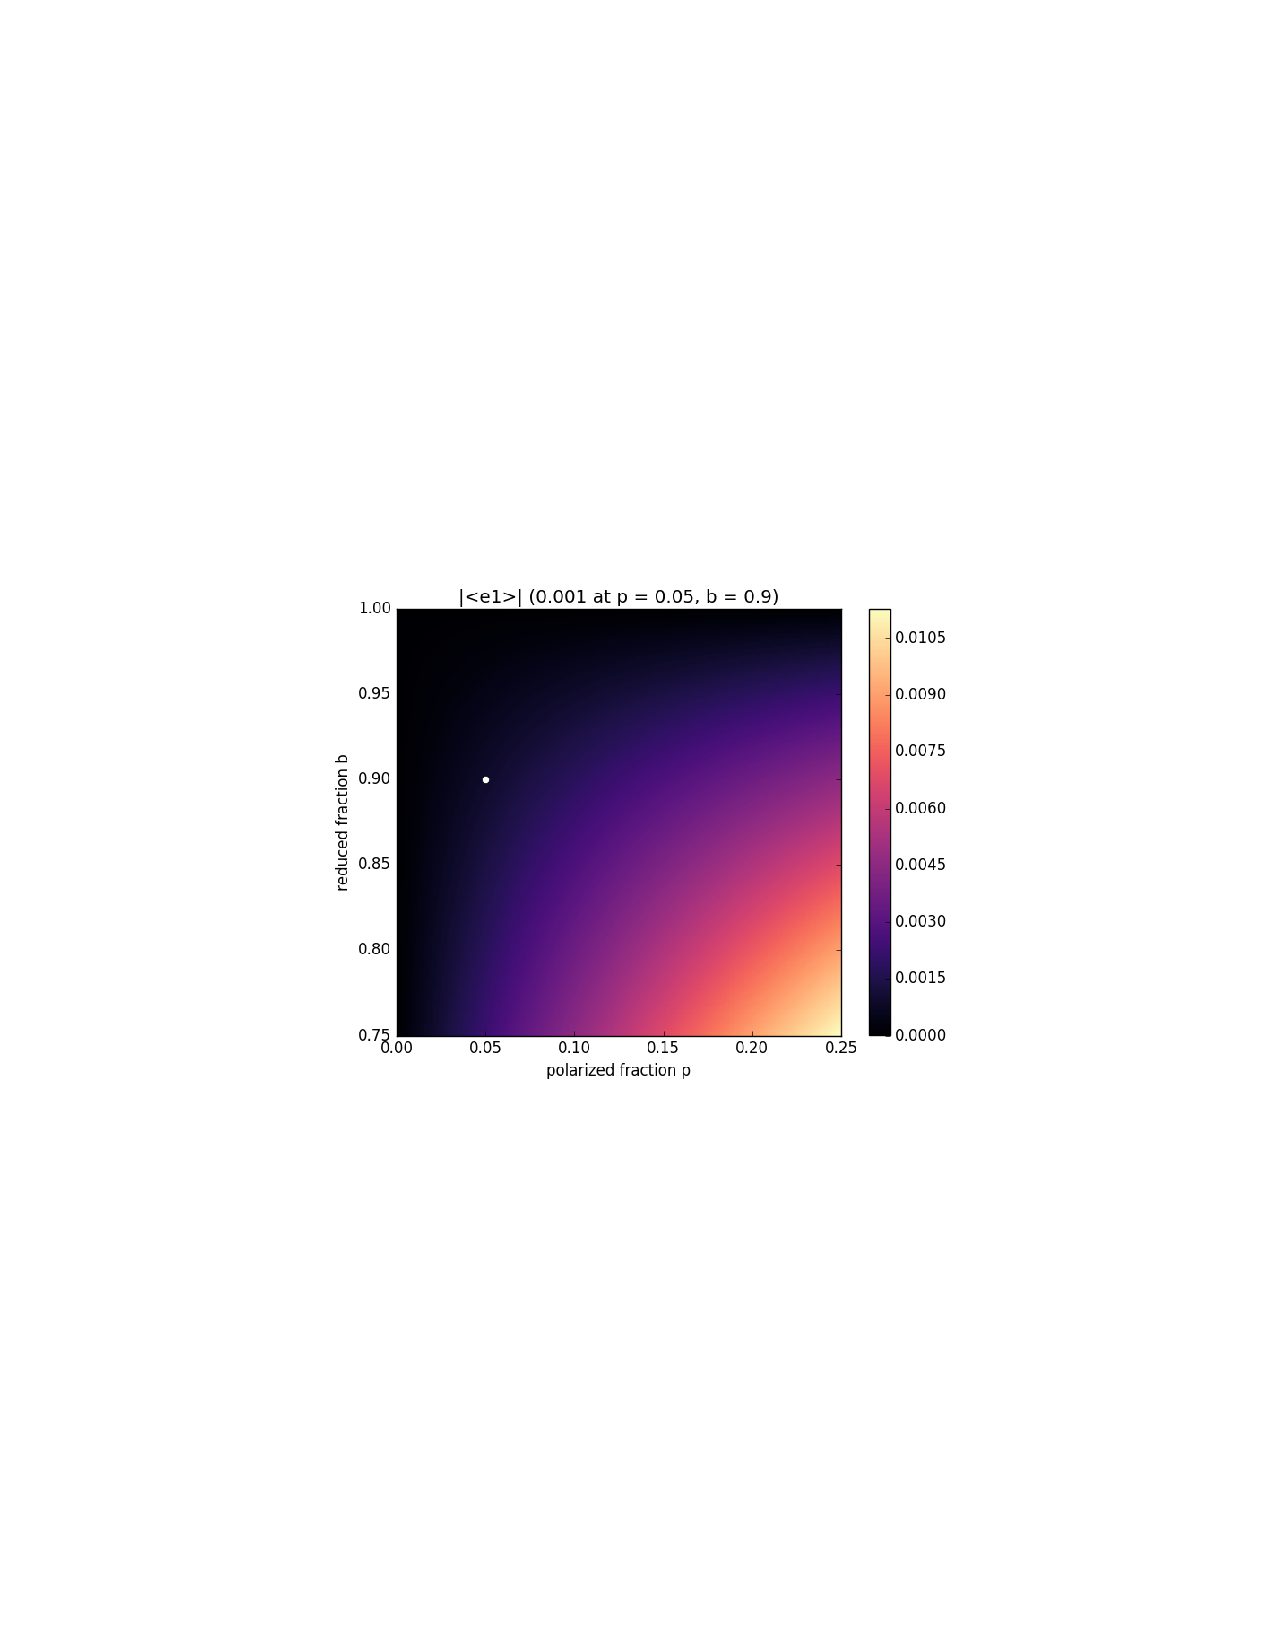
\includegraphics[width=5in]{Plots/polarization-selection.pdf}
\end{center}
\caption{\label{fig:polarization}
The average shear due to weak lensing selection biases due to polarization-dependent quantum
efficiency, as a function of the fraction of polarized light from edge-on disks (horizontal axis)
and the fractional attenuation of the perpendicular polarization (vertical axis).  The dot at
$(0.05,0.9)$ is our fiducial point in parameter space, and has $\langle e\rangle \approx 0.001$.
}
\end{figure}

Another possible polarization-related systematic is a polarization-dependent PSF.  That will be the
subject of future work.

\subsubsection{Interpixel capacitance requirements}

The WFIRST detectors will suffer from electrical crosstalk between the pixels, unlike the optical
 detectors that are based on CCDs. This effect, known as the \emph{interpixel capacitance} (IPC),
 appears as a systematic effect in the weak lensing shear measurements and causes a 
 bias in the measurements if not properly taken into account. The effect of IPC on the point-spread
 function (PSF) was already studied by members of our SIT in \cite{Kannawadi2016}, and requirements were placed
 on the level of uncertainty in the IPC based on how that uncertainty affects the PSF. 

More recently, in late 2016, members of our SIT (Mandelbaum and student Kannawadi) carried out and
analyzed simulations to determine whether additional requirements on IPC are needed to ensure that
weak lensing shear estimation is not biased beyond our tolerances.  To calibrate the shear
multiplicative bias to an accuracy of $2\times 10^{-3}$, we find that the requirements on the IPC
placed by the PSF requirements are sufficient, so no new requirement is needed.  A paper on this
result is in preparation.


\subsection{Photometric Calibration}
\label{sec:wl_calibration}
%================================================
\Auth{Nikhil, Chris}

Our SIT has been instrumental in the Calibration Working Group, since precision cosmology measurements depend sensitively on calibration; subtle effects that might not be noticeable in other areas of astrophysics can become important when trying to measure galaxy shapes to $<0.1$\%. Activities over the past year have included:
\begin{list}{$\bullet$}{}
\item
{\em Dark filter:} Co-I's Wang, Capak, and Hirata participated extensively in the analyses and discussions that led the FSWG to recommend a dark position in the element wheel on WFIRST.
\item
{\em Calibration plan}: Our SIT has contributed extensively to the WFIRST WFI Calibration Plan, including detailed quantitative assessments of calibration approaches and their ability to meet requirements. In some areas, such as dark current and the point spread function, our contributions to the calibration plan are now traceable all the way from science measurements (WL shear) down to the specific calibration approaches and the hardware stability requirements needed for them to work. A major area of work leading up to SRR/MDR is to complete this flow-down for the other areas of calibration.
\item
{\em Detector characterization}: We have made use of the H4RG data provided by the Detector Characterization Laboratory to measure some of the non-linear effects relevant to weak lensing in real H4RG detectors. This is an important practice step toward building calibration pipelines that will support WL science.
\end{list}
In what follows, we provide some highlights from our calibration activities. The list is not exhaustive.

\subsubsection{Dark filter}

In the summer and fall of 2016, the FSWG was tasked with determining whether a dark filter was needed for WFIRST calibration. This required the FSWG to enumerate the list of calibration tests that might use the dark filter, and establish whether alternative options were possible. We led the effort to assemble this list of tests based on input from the SITs (both ours and others), the SOC, and  Project personnel. The list\footnote{\tt DarkAlternativesMatrix\_161030.docx} included 14 items: (i) the dark current (including internal instrument backgrounds); (ii) unstable pixels; (iii) post-reset transients; (iv) read noise correlations; (v) inter-pixel capacitance; (vi) gain measurement; (vii) the high spatial frequency flat; (viii) the low spatial frequency flat; (ix) persistence from previous observations; (x) persistence from slews; (xi) classical linearity; (xii) count rate dependent non-linearity; (xiii) the brighter-fatter effect; and (xiv) persistence re-activation.

The problem of persistence from slews (i.e.\ streaks across the detector following a slew from one observation to another) is of particular importance to weak lensing, because it leads to a coherent, highly directional pattern on the detector that has the correct symmetry to induce a coherent systematic error in the galaxy ellipticities. This is a concern without a dark capability, or even with a dark capability if it is not (or cannot be) used during every slew. Our group identified two budgets in WL that flow down into slew persistence requirements. First is the total systematic shear error budget of $2.7\times 10^{-4}$. Second is the masked pixel budget.

The details of the slew persistence study are provided in the Calibration Plan. It consisted of several stages: first, assessing the magnitude distribution of the stars that would be encountered in the High Latitude Survey; then assessing the probability of stimulus levels in a slew, given the distribution of slews from our operations model (\S\ref{sec:operation}); and then folding this through a persistence model (based on DCL data for the development H4RG detectors) to predict the probability distribution of persistent pixels in the HLS imaging survey. The stimulus distribution ($x$ in e: the well depth to which a pixel is filled during a slew) from the Calibration Plan is shown in Figure~\ref{fig:slewcompare}, and the persistence signal distribution ($y$ in e: the persistence signal in a pixel over the course of an exposure) is shown in Figure~\ref{fig:sp_cdf}.

\begin{figure}
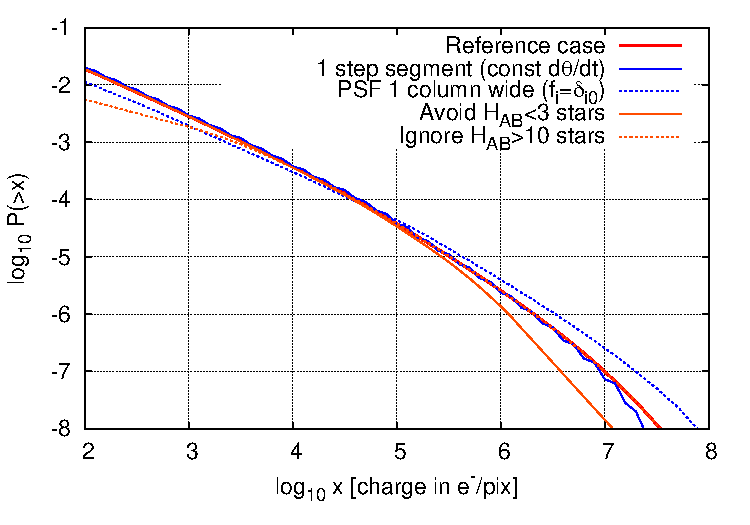
\includegraphics[width=5in]{Plots/slew_compare.pdf}
\caption{\label{fig:slewcompare}Comparison of stimulus levels predicted
under different assumptions and approximations. The vertical axis
shows the log probability to exceed a given stimulus level during a
slew of 0.4 degrees (a step along the short axis of the field,
executed frequently during the HLS). The thick red line indicates
reference assumptions. The solid blue line treats the slews as being
at constant $\dot\theta$. The dashed blue line approximates the PSF as
1 column wide (all the flux from the star is concentrated in the
central column). The orange lines show what happens if bright ($H_{\rm
AB}<3$) or faint ($H_{\rm AB}>10$) stars are excluded from the model.}
\end{figure}

\begin{figure}
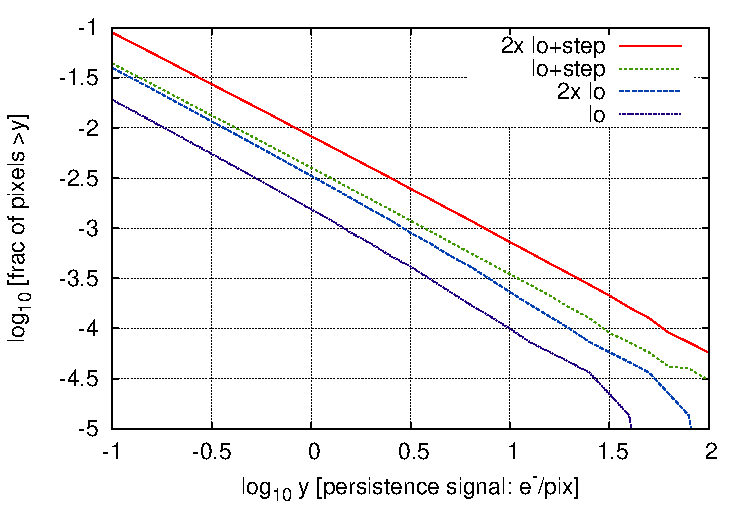
\includegraphics[width=5in]{Plots/sp_cdf.pdf}
\caption{\label{fig:sp_cdf}The cumulative distribution function of slew-induced persistence in the HLS imaging survey, $P(>y)$.
The persistence signal $y$ is estimated in electrons per pixel; the decaying persistence curve is integrated over a 160 s. Several persistence models are shown, including the ``lo'' case (typical of the development detectors), and a ``lo+step'' case (including an order of magnitude step at saturation, as seen in portions of some detectors). This figure has not been updated yet to go from the 6-year to the 5-year observing plan, although we expect only minor differences.}
\end{figure}

After negotiating with the Project, we settled on a mitigation strategy for slew persistence that involved saving the spacecraft orientation information from the Attitude Control System (ACS), using this to predict the locations of persistence from bright star streaks, and masking $\pm2\sigma$ on either side of these streaks. Unmasked streaks are simply accepted as part of the systematic error budget. Their impact on shape measurement is based on an analytic result derived by our SIT and tested against Monte Carlo simulations:
\begin{equation}
\Delta \gamma_1 + i\Delta \gamma_2 = \frac{M\Omega_{\rm
max}\sigma_{\rm n}^2 R^4}{2F^2N_{\rm ind}\,{\rm Res}} f_{\rm scale}
f_{\rm aniso},
\label{eq:dg}
\end{equation}
where $\Delta\gamma_{1,2}$ are the two components of spurious shear; $M$ is a margin factor; $\Omega_{\rm max} = 421.3$; $\sigma_{\rm n}^2$ is the variance of the persistence image; $R$ is the radius of the galaxy in pixels; $F$ is the signal from the galaxy in electrons per exposure; $N_{\rm ind}$ is the number of {\em independent} exposures of the galaxy\footnote{This may be less than the total number of exposures of the galaxy, since slew persistence from successive exposures will be correlated.}; Res is the galaxy resolution factor \cite{Bernstein2002}; $f_{\rm scale}$ and $f_{\rm aniso}$ are factors $\le 1$ describing the scale dependence and anisotropy of the persistence power spectrum (defined to be 1 in the worst case).

The results of this study -- shown in Figure~\ref{fig:slew_results_oct16} -- are promising, given the top-level systematic shear budget of $2.7\times 10^{-4}$ and that the modern detectors typically show ``lo'' or (in some regions) ``lo+step''-like behavior, rather than the much larger persistence characteristic of the WFC3-IR model (third column). The masking algorithm will continue to be revisited as part of the mission optimization. However, the small number of masked pixels led the FSWG to conclude that a dark shutter that operated during every slew was not required for the WFIRST HLS.

\begin{figure}
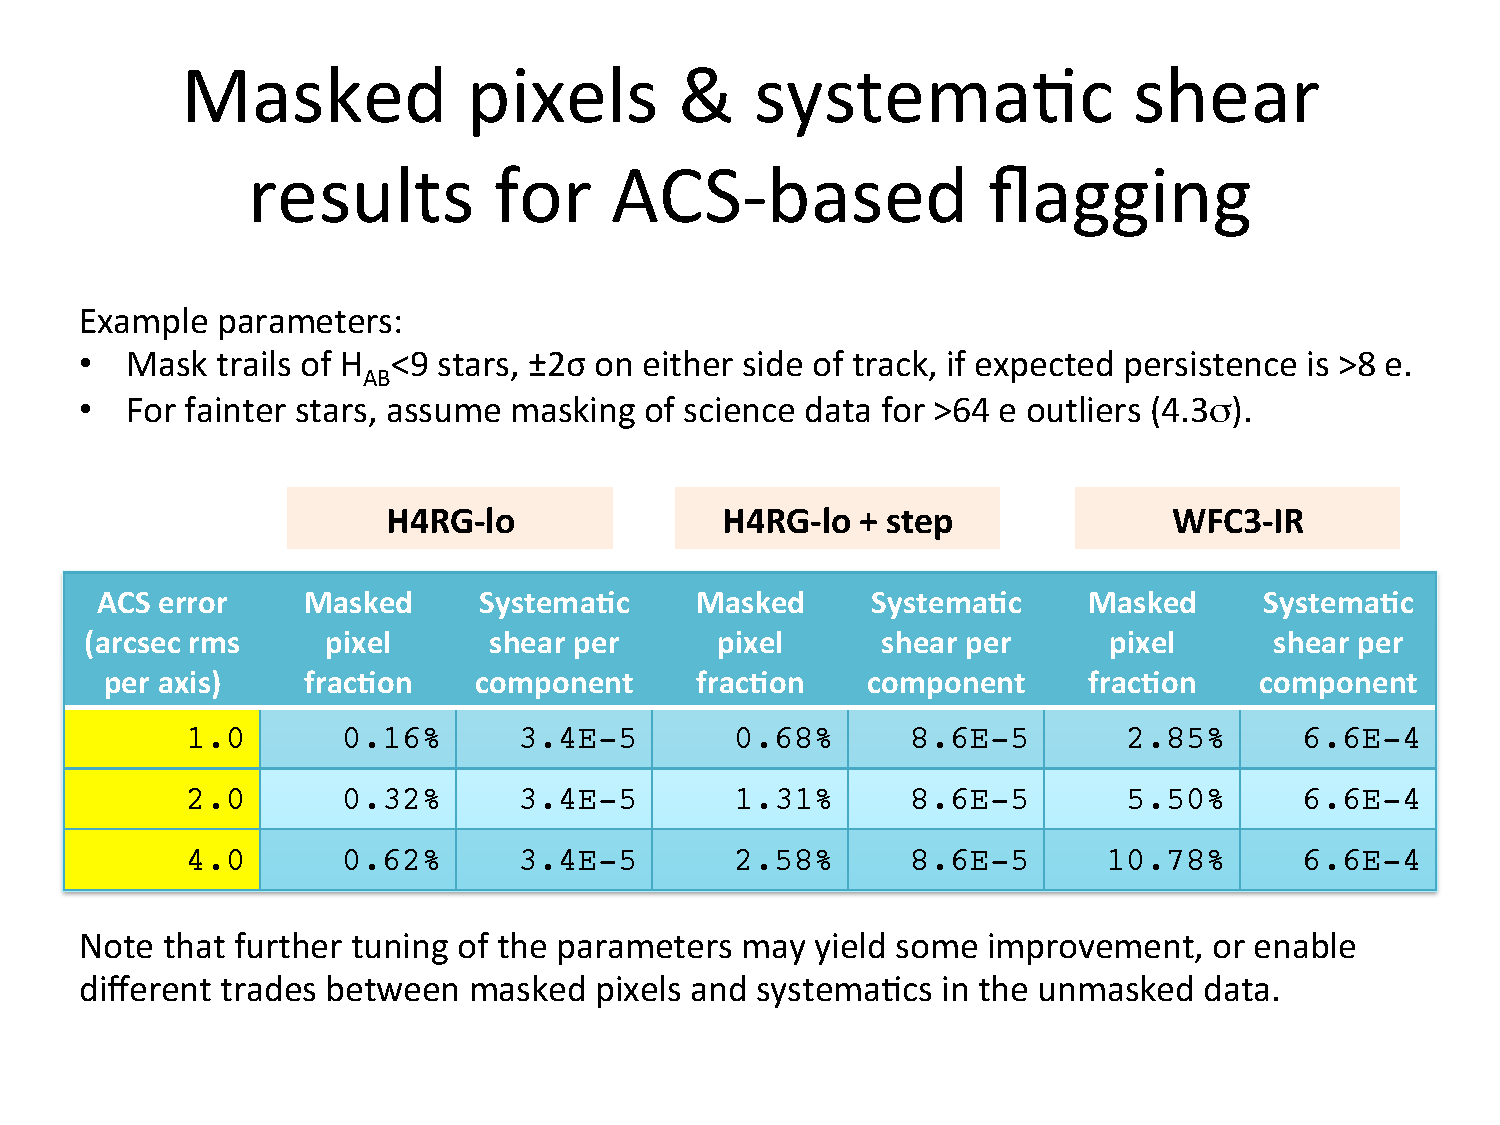
\includegraphics[width=5in]{Plots/slew_results_oct16.pdf}
\caption{\label{fig:slew_results_oct16}The outcome of the October 2016 slew persistence study. This shows the masked pixel fraction and the predicted systematic shear due to unmasked streaks as a function of both the persistence model and the accuracy of pointing information.}
\end{figure}

We carried out a related study, also using Eq.~(\ref{eq:dg}) and related machinery, to assess how well we need to know the dark current for WFIRST. Dark current measurements without a dark filter are possible, e.g.\ via median algorithms that combine many exposures from a survey, but are subject to: (i) a degeneracy in which the ``true'' sky brightness is unknown and hence the zero level of the dark current cannot be established, and (ii) possible correlated errors from imprinted celestial sources. The requirements, as derived in the appendix to the calibration plan, are:
\begin{list}{$\bullet$}{}
\item The error in the dark current + bias determination in a 140 s
HLS imaging exposure shall be no more than $0.0096f_{\rm corr}^{-1/2}$
e/p/s (uncorrelated part) or $0.0017 f_{\rm corr}^{-1/2}$ e/p/s
(imprinted celestial sources).
\item The error in the dark current + bias determination in a 297 s
HLS spectroscopy exposure shall be no more than $0.0059 f_{\rm
corr}^{-1/2}$ e/p/s (uncorrelated part) or $0.00072 f_{\rm
corr}^{-1/2}$ e/p/s (imprinted celestial sources).
\end{list}
Here ``$f_{\rm corr}$'' denotes the factor by which we plan to correct biases induced by errors in the dark current map (we normally choose $f_{\rm corr}=1$ to be conservative). The requirements are traceable to additive shear biases from non-circular imprinted celestial sources; multiplicative shear biases as the noise in the dark current map results in e.g.\ galaxy centroids getting ``pulled'' toward pixels whose measured dark current fluctuates below the true dark current of that pixel; and Eddington-like biases for sources detected in the GRS. While the semi-analytic estimates in the calibration plan based on source counts suggest that the HLS imaging requirement can be met without a dark filter, our SIT and the Calibration Working Group had concerns about possible degeneracies in the self-calibration procedure that can only be addressed by a detailed simulation. Moreover, the approach requires empty space in the images, which we will not have in the case of grism spectroscopy. As the imaging exposures are shorter than the spectroscopy exposures, this would require dedicated long imaging exposures (of HLS spectroscopy exposure length) just for the purpose of self-calibrating the dark. Due to sky Poisson noise, we would need many of these images -- our Feburary 2017 estimate was for $N=73$ exposures, which, if done every week, would consume 4\%\ of the wall clock time. In light of these and other issues, the Calibration Working Group recommended that WFIRST maintain the dark filter.

\subsubsection{Calibration plan}

Our SIT has contributed extensively to the WFIRST WFI Calibration Plan. This includes extensive quantitative analysis of proposed calibration techniques, as detailed in the appendix to the plan. Some highlights follow.

The requirement on knowledge of the dark current and the calibration approaches are fully defined, based on analysis done during the dark filter trade (October 2016 -- February 2017).

Weak lensing was found to place demanding requirements on measurement of the count rate-dependent non-linearity (CRNL). The weak lensing program is sensitive to CRNL because it enhances the bright center of a PSF star relative to its wings, thereby making the star appear slightly smaller, but does not have a similar effect on the faint galaxies used for shape measurement. The PSF second moment is biased by a factor of $1-\alpha$ (where $\alpha$ is the CRNL exponent), and has a top-line systematic error budget of $7.2\times 10^{-4}$. This means that if $\alpha$ is measured to $\pm 3\times 10^{-4}$ (the requirement from the supernova SITs), then CRNL consumes 17\%\ of the PSF size error budget, in an RSS sense. Given that CRNL is a pernicious bias for two of the dark energy probes, we recommended a multi-faceted approach to CRNL calibration, including a lamp-on/lamp-off capability for WFIRST (this was not available on WFC3-IR).

Our team has revisited the wavefront stability requirements for weak lensing, using a set of codes and scripts on the team's GitHub site. This begins with a Fisher matrix analysis of the uncertainties in the shear power spectrum, and our top-line requirement that the systematic errors be equivalent to the statistical errors even if the survey is extended to 10,000 deg$^2$ (i.e.\ in an RSS sense, the systematic errors should be 20\%\ of the statistical errors in the nominal 2,000 deg$^2$ survey). Requirements are assessed using the significance, defined by
\begin{equation}
Z = \sqrt{\Delta{\bf C}\cdot{\bf\Sigma}^{-1}\Delta{\bf C}},
\label{eq:alpha}
\end{equation}
which is the number of sigmas at which one could distinguish the correct power spectrum from the power spectrum containing a systematic error. We built sub-allocations for multiplicative (shear calibration) errors, and for additive (spurious shear) errors in each angular bin. An early discovery was that this process depends on the redshift dependence of the shear error: some redshift dependences are ``worse'' than others by the $Z$-metric. The worst possibility is {\em not} for the error to be redshift-independent, but rather for it to change sign, as this can mimic a change in redshift evolution of the growth of structure.

In our current formalism, for each angular template, we introduce a limiting amplitude $A_0^{\rm flat}(\alpha)$, defined to be the RMS spurious shear per component $A_0$ at which we would saturate the requirement on $Z(\alpha)$ for angular bin $\alpha$ in the case of a redshift-independent systematic $w_i=1\,\forall i$ (here $\alpha$ denotes an angular bin and $i$ a redshift bin). That is, if the additive systematics did not depend on redshift, we could tolerate a total additive systematic shear of $A_0^{\rm flat}$ (RMS per component) in band $\alpha$. We also introduce a scaling factor $S[{\bf w},\alpha]$ for a systematic error
\begin{equation}
S[{\bf w},\alpha] = \frac{Z(\alpha) \,{\rm for\,this\,}w_i}{Z(\alpha)\,{\rm for\,all\,}w_i=1}
\end{equation}
that depends on the redshift dependence $w_i$. An additive systematic error that is independent of redshift will have $S=1$. A systematic that is ``made worse'' by its redshift dependence will have $S>1$, and a systematic that is ``made less serious'' by its redshift dependence will have $S<1$. The requirement that the (linear) sum of $Z$s not exceed $Z(\alpha)$ thus translates into
\begin{equation}
\sum_{\rm systematics} [A(\alpha)]^2\times S[{\bf w},\alpha] \le [A_0^{\rm flat}(\alpha)]^2,
\label{eq:A-S-sum}
\end{equation}
where $A(\alpha)$ is the RMS additive shear per component due to that systematic. We take the ``reference'' additive shear to be the additive shear in the most contaminated redshift slice; in this case, $w_i=1$ for that slice, and $|w_i|\le 1$ for the others. Under such
circumstances, we can determine a {\em worst-case scaling factor} $S_{\rm max,\pm}(\alpha)$, which is the largest value of $S[{\bf
w},\alpha]$ for any weights satisfying the above inequality. We may also determine a worst-case scaling factor $S_{\rm max,+}(\alpha)$
conditioned on $0\le w_i\le 1$, i.e.\ for sources of additive shear that have the same sign in all redshift bins. In most cases, however, something is known about the redshift dependence of the systematic error (e.g.\ for PSF errors the error scales with the size of the galaxy, and hence has a redshift dependence tied to the measured redshift evolution of galaxy sizes). In these cases, we use the correct redshift weighting factor $S$. This approach has been critical in order to set stability requirements that are consistent with the Project's integrated modeling results.

We have begun incorporating the HLS observing strategy (\S\ref{sec:operation}) in studies of self-calibration of time-dependent drifts in the response of the system (i.e.\ time dependence of the conversion from $\mu$Jy on the sky to DN/s in the digitized detector system outputs). This model is in a state of flux as we add parameters to it, but here we show a current snapshot allowing for time-dependent drifts of the response of each of the 18 SCAs making up the focal plane, with time dependence parameterized in calibration periods of $\Delta t$ (assessed down to a period of 3 hours) each. Both individual-SCA drifts and common-mode drifts are allowed, with an assumed intrinsic variation (calibration prior) of 1\%\ RMS drift in each $e$-fold of timescales. A network of randomly distributed stars with a density of 500 stars/deg$^2$ and $S/N=50$ was assumed; in self-calibration, the magnitudes of these stars are {\em not} known a priori, but are assumed to be stable across multiple repeated observations of the same field. These are preliminary parameters being used to test our tools and are not currently held as requirements. The stellar density model is very conservative since the Trilegal model predicts star counts of 572, 803, 990, and 1137 stars/deg$^2$ at $H_{\rm AB}=18-19$, $19-20$, $20-21$, and $21-22$ at the SGP, and even an $H_{\rm AB}=22$ star will have $S/N>50$. The temporal stability of the system needs further study and will be varied as an input parameter in future versions of this model. The current model uses the April 19, 2017 update to the HLS observing strategy. The number of calibration parameters varies depending on the filter, since there are no parameters for periods of time when the instrument is not observing in that filter; the current version has 17262 parameters for the H band.

Despite the intrinsic stability assumed, in which each SCA can have its response fluctuate by 1.67\%\ RMS from one time interval to the next, the repeated observations do an excellent job of tracking these changes and reducing the posterior uncertainty. Even for $\Delta t = 0.125\,$days$=3\,$hours, the posterior calibration errors are at the level of 0.14--0.17\%\ RMS (here ``RMS'' is weighted by number of observations), depending on the filter.  An example of the model output (predicted uncertainties in the calibration parameters for each SCA at each epoch) is shown in Figure~\ref{fig:hcalfig}. It must be remembered that this analysis is overly simplistic in some ways -- particularly that we have not yet allowed for shorter-timescale variations (i.e.\ on timescales $<\Delta t$), nor have we allowed for separate gain drifts among the different readout channels. These will have to be included in a future version of the model. On the other hand, the stellar density and $S/N$ assumptions were extremely conservative (e.g.\ the full range of stellar magnitudes 18--22 should have 7 times more stars than were assumed, even at the Galactic pole), so there is margin to absorb these additional degrees of freedom. The next iteration of the model for time-dependent calibration drifts will include additional parameters, as well as updated priors reflecting expected detector system stability rather than the place-holder requirements shown here.

\begin{figure}
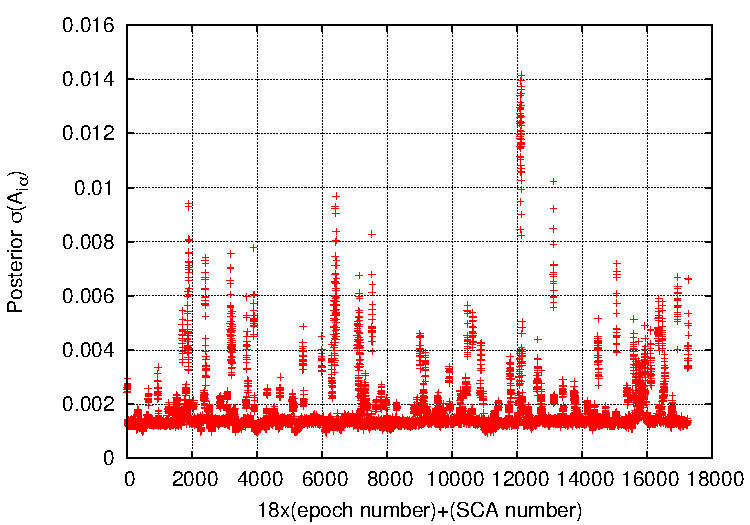
\includegraphics[width=4.5in]{Plots/hcalfig.pdf}
\caption{\label{fig:hcalfig}An example of the posterior calibration error from an HLS self-calibration calculation. The horizontal scale displays the time intervals (left-to-right in time order), with 18 points per time interval indicating the various SCAs. The vertical axis shows the standard deviation of the calibration solution for that SCA at that time, $\sigma(A_{i\alpha})$, relative to the survey mean. The figure shows the case of H band with $\Delta t = 0.125$ days. This example had 17262 calibration parameters. A few epochs, mostly containing only a few observations, are poorly constrained due to minimal overlap observations. It is subject to refinement and the input parameters of the model will be varied as we work toward requirements on the stability of the detector system.}
\end{figure}

\subsubsection{Detector characterization}

The WFIRST dark energy analyses will place enormous demands on our understanding of the detectors. Some aspects of this problem can be anticipated in advance -- for example, we know that effects such as inter-pixel capacitance, count-rate-dependent non-linearity, etc.\ will need to be carefully characterized, and we are working as part of the Calibration Working Group to build these measurements into the mission. However, with systematic error budgets at the level of a few$\times 10^{-4}$, it is likely that WFIRST analyses will turn up new effects that were not apparent in past missions. Therefore a key task for our SIT is to analyze the data from development detectors and identify these new effects early enough to inform the calibration plan.

In ground-based weak lensing projects using thick CCDs (e.g.\ DES), one of the key detector issues has been the {\em brighter-fatter effect} (BFE). This is an electrostatic effect in which as a pixel fills up with collected charge, it changes the electric field geometry and new charges generated are more likely to be deflected into neighboring pixels. This has the effect of making bright stars appear larger than faint stars, as the repulsion effect is non-linear and increases with signal level. The field geometry is very different in a NIR detector, but a brighter-fatter effect is still possible.

We have searched for the brighter-fatter effect in the H4RG detector arrays using the flat fields for two devices H4RG-17940 and H4RG-18237, provided to us by the DCL. The BFE imprints a signature in the auto-correlation function of a flat field; using the correlations in multiple non-destructive reads in a flat field, one can separate linear IPC from the BFE. Preliminary brighter-fatter effect results for H4RG-17940 are shown in Figure~\ref{fig:kernel}. The BFE coefficients are $a'_{\Delta i,\Delta j}$, which is the fractional change in effective area of pixel $(i,j)$ when an electron is placed in pixel $(i+\Delta i, j+\Delta j)$; they have units of parts per million per electron (ppm/e). The flat auto-correlations are sensitive to both the brighter-fatter effect and non-linear inter-pixel capacitance (NL-IPC); we are currently working on distinguishing the two effects.

\begin{figure}
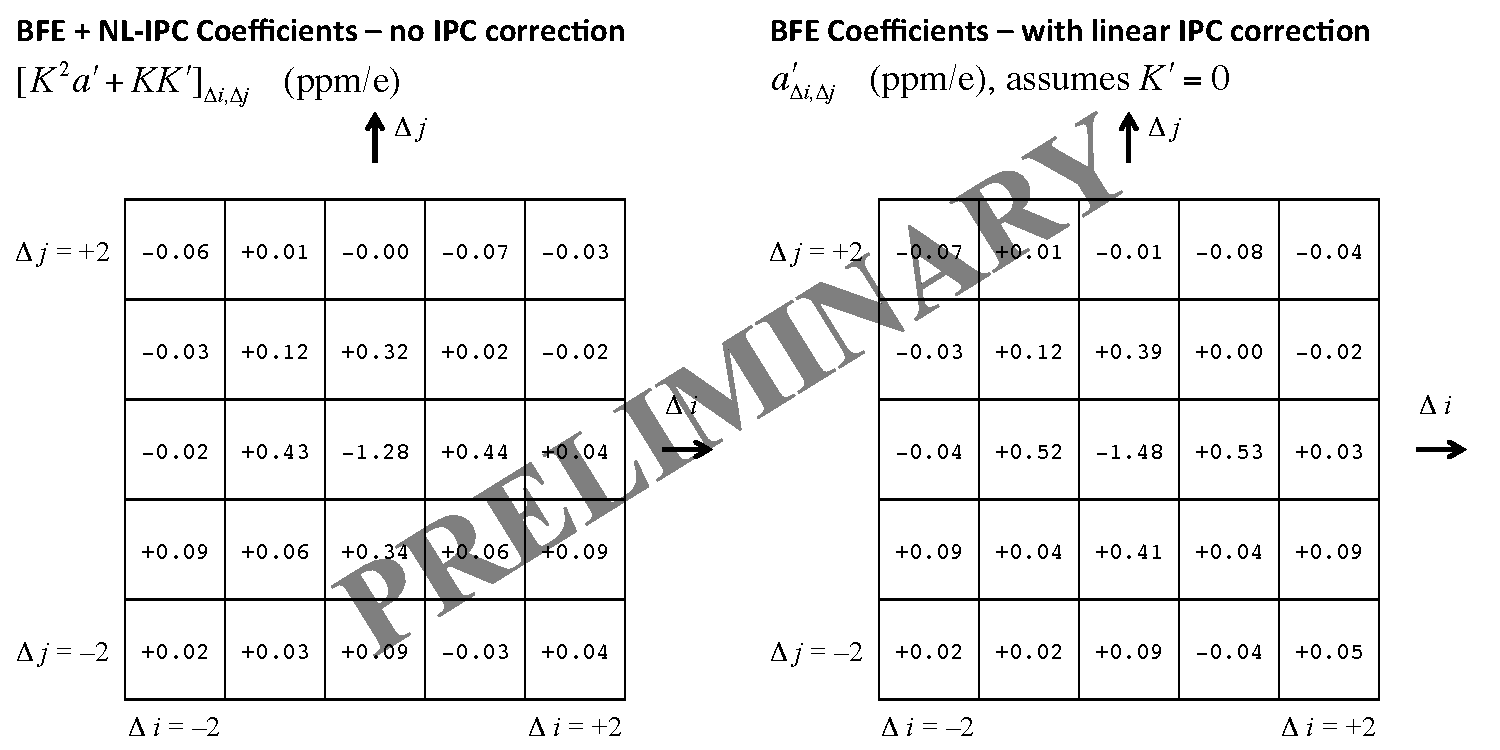
\includegraphics[width=6.2in]{Plots/kernel-17940B.pdf}
\caption{\label{fig:kernel}The BFE + NL-IPC coefficients $[K^2a'+KK']_{\Delta i,\Delta j}$ (left panel) and IPC-corrected coefficients $a'_{\Delta i,\Delta j}$ (right panel), for H4RG-17940. Note that the IPC-corrected coefficents assume that the IPC is linear, i.e.\ the non-overlapping correlations are ascribable entirely to the BFE and not NL-IPC. The $1\sigma$ uncertainty in each pixel is 0.07 ppm/e.}
\end{figure}

\comment{
Achieving a uniform photometric calibration of the survey is an essential requirement
for achieving the scientific goals of WFIRST, since calibration variations on large
scales can swamp the cosmological signals and make dedicated photo-$z$ calibration
fields unrepresentative of the whole survey.
Our calibration requirements and
strategy development will be led by Co-I Padmanabhan, the chief
architect of the ``uber-calibration'' method used for the SDSS \cite{Padmanabhan2008};
members of our team also have experience designing calibration strategies for
Euclid and LSST.  Co-I Capak is an active member of the Euclid calibration team. Co-I Lupton plays a
key role in designing LSST and HSC calibration strategies.
Using our simulations and forecasting tools, we will determine both
absolute and relative calibration requirements for the survey as a function
of angular scale on the sky. Based on these requirements, we will
define a calibration plan for WFIRST, including overlapping regions
for self-calibration over the entire survey and repeated fields or use of
the microlensing survey data for small scale calibration (e.g., flat fields
and intra-pixel response).  We will also define methods and metrics for
tracking the photometric stability and calibration quality
across the survey.
We will determine formats for making the calibrations and calibration
error maps publicly available to enable related analyses.
We will pay special attention to the relation of the photometric calibration
strategy to instrument design, including the impact of field-dependent bandpass
variations and NIR detector effects such as persistence and rate-dependent nonlinearity.
We will track which such effects can be measured internally to the WFIRST data, and
when dedicated observing modes might be needed (such as observations of the sky with
an internal illumination source also on). The latter considerations will feed into
the observing strategy and hardware requirements.
}

\subsection{Photometric Redshifts}
\label{sec:wl_calibration}
%================================================
\Auth{Peter, Shooby, Dan}

Accurate photo-$z$s are crucial to all WFIRST probes of
dark energy. We plan to combine calibrations of the color-redshift relation
\cite{Masters2015} and cross-correlation techniques to achieve the
required photo-$z$ performance. These will be supplemented by
consistency checks such as the expected level of WL cross-correlations
for sources in different photo-$z$ bins.
Our team is actively developing the color-redshift mapping for WFIRST
(supported by WFIRST Preparatory Support (WPS); PI Capak),
with initial tests demonstrating a path
to meeting the WFIRST requirements on photo-$z$ bias. Our team has worked with NASA HQ
to allow the NASA Strategic Keck Proposals to obtain the required spectra.
A key piece of the proposed work will be carrying out these spectroscopic surveys.
Cross-correlation methods \cite{2008PhRvD..78d3519H, 2008ApJ...684...88N, Menard2013, Newman2015} require
spectroscopic overlap and rely on assumptions about the bias of galaxies. We
will determine the applicability of these methods and their implications for
survey design. We also plan
to investigate promising new methods of photo-$z$ inference \cite{Bordoloi2010, Jasche2012, Benjamin13}
as additional consistency checks.

Our team will refine the performance estimates and calibration data requirements for each of
these photo-$z$ methods. This will include studying the impact on WFIRST operations
(e.g., incorporating observations of spectroscopic calibration fields in the observing plan).
Co-I Capak will lead the photo-$z$ effort, with support from other team members (Mandelbaum, Hirata,
Hudson, Jain, Eifler, Krause, Miyatake) who have extensive experience
using photo-$z$ calibration techniques for WL applications with SDSS
(e.g., \cite{2012MNRAS.420.3240N,2008MNRAS.386..781M}),
Canada-France-Hawaii Telescope (CFHT), DES and HSC survey data.


%{\bfseries C.H.: Need uniform ``primary/secondary/tertiary'' nomenclature. Also discuss photometric calibration requirements.}

%\subsection{Cosmological Forecasting, Methodology Development, and Cosmological Simulations}
\subsection{Cosmological Forecasting, Simulations, and Methodology Development (D2, D8, D9)}
\label{sec:wl_methodology}
%=========================================================================
%\Auth{David W, Tim, Elisabeth, Rachel B, Alina, Bhuvnesh}


\subs{Forecasting.}
Cosmological forecasting plays
an essential role in connecting strategies and requirements defined at
the instrument and observation level to WFIRST's top-level science goals.
Co-Is Bean, Hirata, Padmanabhan, Wang and Weinberg have been
involved in the forecasting for the WFIRST reports and
for cosmological surveys and space missions in general.
One of our early activities will be to develop a forecasting
framework for WFIRST building on Eifler \& Krause's \CoLi, incorporating all of the dark
energy probes from the HLS Imaging, Spectroscopy, and Supernova surveys.
We will incorporate the impact of the leading observational and theoretical systematics
through ``nuisance parameters'' that can be marginalized over in cosmological
parameter estimates.  This framework will be much more thorough
than the one used for the SDT reports, and it will enable complete
flow-down and flow-up analyses between the instrument, strategy, and
software requirements and the expected cosmological performance of
WFIRST.  We will initially use analytic approximations for error covariance
matrices and the dependence of observables on model parameters.  We will
steadily update these approximations using the simulations described below.
For cosmic shear, we will extend existing work on the WL bispectrum
(e.g., \cite{Kayo2013,Fu14}), which should
produce complementary constraints to the power spectrum and may have
similar statistical power given the high source density expected in
HLS Imaging.  Figure~1 illustrates the application of \CoLi\ to WFIRST
multi-probe forecasting.

\subs{Cosmological simulations.} As emphasized in SDT15, WFIRST will improve the statistical precision
of cosmic expansion and structure growth measurements by factors of $5-50$
compared to current data, and will require commensurate improvements in modeling the
lensing and clustering signals  and the astrophysical contaminants thereof.
We will  devote significant effort to modeling the nonlinear regime via a combination of numerical
simulations, perturbation theory, and empirical measurements, to
 address issues such as baryonic effects on matter clustering
\citep{Zentner2013,VanDaalen2014}; the
validity of the Born approximation \citep{Schafer2012}; and galaxy intrinsic
alignments \citep{Hirata2004,Laszlo2011,Krause2015}.
We will develop analysis strategies that take advantage of
our methodological improvements and marginalize over remaining uncertainties.
The computational requirements for cosmological simulations will increase
significantly in the years just prior to launch. Where these resources will
be sourced from is currently an unsolved issue that is being investigated at
the project level. Co-I Kiessling has been part of this effort at the request of
the project and she will be responsible for leading
the team efforts to quantify computing requirements beyond FY20.
% and to develop techniques to reduce them.
%
% RM took a bunch of long specific sentences and made this more general one.
%For cosmic shear, we will develop
%``self calibration'' strategies to eliminate biases and mitigate statistical
%losses from uncertainties in shear calibration and \photoz\ error
%distributions.  These strategies will be developed in concert with
%and informed by the methods and tests discussed previously in
%\S\ref{sec:wl_requirements} and~\ref{sec:wl_methodology}.
%We will use cosmological N-body simulations and hydrodynamic
%simulations to predict non-linear matter clustering at the accuracy
%needed for WFIRST modeling, including the impact of realistic
%treatments of baryonic physics (see, e.g., \cite{Zentner,VanDaalen,Etc}).
%We will apply ray tracing to cosmological simulations to test
%for biases such as due to the ``Born approximation'' typically used in weak
%lensing analysis, and to calibrate any necessary corrections.
%We will use hydrodynamic simulations, perturbation theory calculations,
%and empirical information to sharpen predictions of galaxy intrinsic alignment,
%one of the main theoretical systematics for cosmic shear.

%\textbf{Bhuv: The two paras below describe a very broad program. If not essential, perhaps better to make it shorter and less sweeping. Also, is the connection to image simulations ok?}
%Our methodology development and tests will make heavy use of cosmological
%simulations.
Most of our work will use large-volume $N$-body simulations (gravity only) in concert
with statistical recipes or semi-analytic models for assigning
galaxies to dark matter (sub-)halos. A large set of such simulations ranging in size from tens of billions to a trillion particles already exists. These will be made available to the collaboration by collaborator Heitmann and will be augmented over time with more simulations as needed.
We will use hydrodynamic simulations
of smaller volumes, provided by collaborator Yoshida, for targeted investigations such as the impact of
baryonic physics on the matter power spectrum or as a realistically
complicated test of non-linear galaxy bias models.
From the $N$-body simulations we will produce mock galaxy catalogs
both in fixed redshift cubes and in light cones with realistic survey
geometry and redshift evolution.
We will use these mocks to understand the effect of observational complications
(survey geometry, variable depth and completeness, etc.) on WL and clustering
measurements and to provide realistically clustered inputs for the pixel-level
simulations described earlier.

% C.H. -- I would really like this but it's very ambitious and not clear that it is
% higher priority than subsets of the HLS simulated at very high fidelity.
% By the end
%of the 5-year investigation period, we aim to produce several complete
%realizations of the full pixel-level HLS data set.

%The overall cosmological simulation effort is large, but many ambitious
%dark energy experiments face a similar challenge.
Our team includes
Co-I Kiessling and collaborators (Heitmann, Takada, Yoshida) who are leading similar efforts
for Euclid, Subaru HSC and PFS, DES, DESI and LSST. In \S
\ref{sec:fac_equip} we describe the computing facilities that will
enable these computations.
%By 2020, advances in computing will make it possible to run larger numbers of simulations, or explore more parameter space at a given size and resolution.
We will publish papers documenting our methodology development and
will simultaneously release the associated simulations.
This growing library of publicly available simulations will encourage
the broader community to develop analysis strategies that will
ultimately be applied to WFIRST (and other surveys).
%While we expect major advances over
%the 5-years of this SIT, we do not expect to solve all of the modeling
%challenges in this period.  One of our deliverables will be a list of remaining (post-CDR) tasks
%to address the remaining modeling uncertainties.

%\setlength\intextsep{-2pt}
%\begin{center}
%\begin{wrapfigure}{r}{1.0\textwidth}
\begin{figure}[!t]
 \begin{boxedminipage}{1.0\textwidth}
 \begin{center}
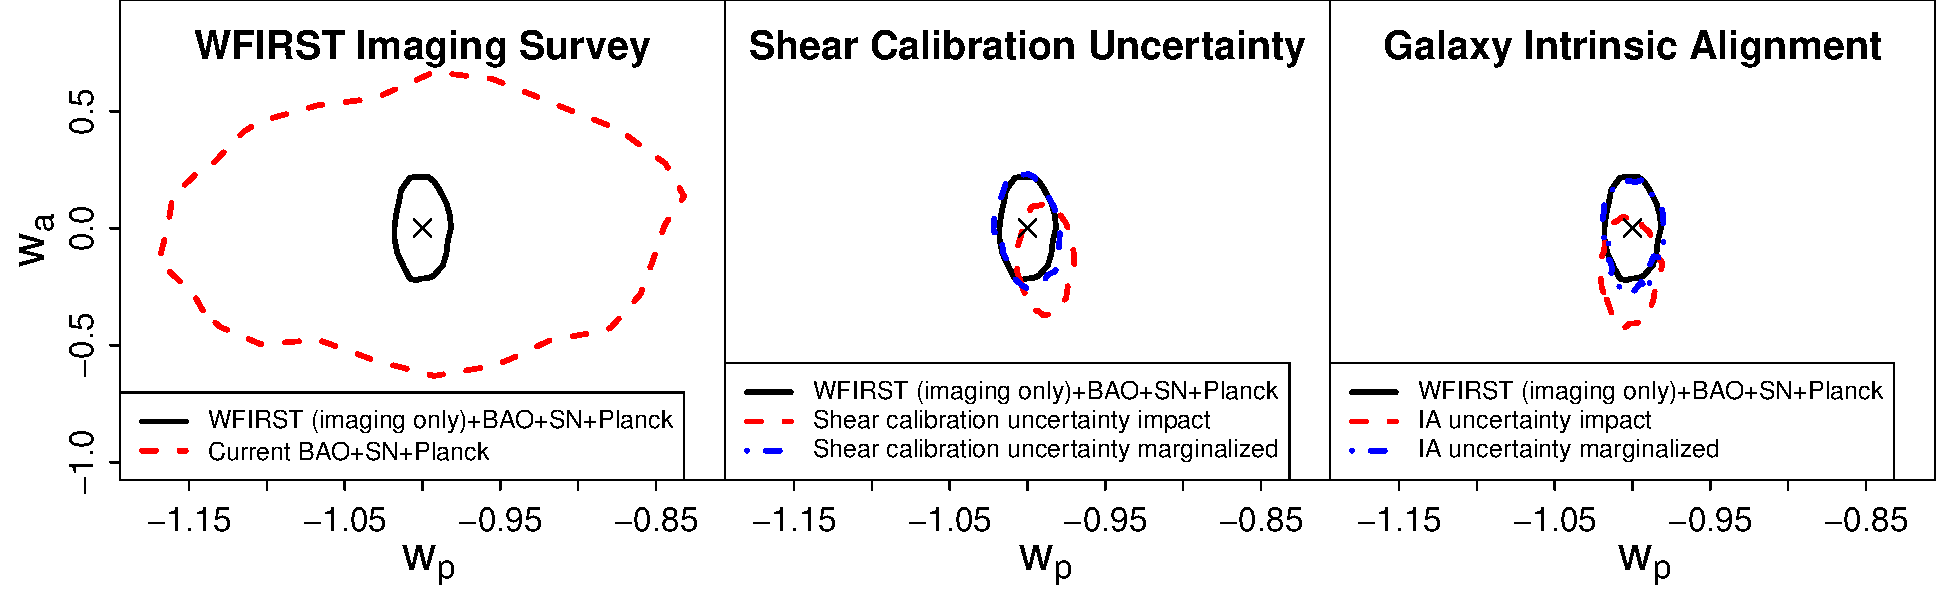
\includegraphics[width = \textwidth]{Plots/WFIRST_combi_forecasts.pdf}
\label{fig:WLsys}
 \end{center}
\vspace{-1.25cm}
\caption{\footnotesize{\CoLi\ forecasts of constraints on the dark energy equation-of-state
from combining current CMB+BAO+Supernovae (SN) data with anticipated WFIRST WL, GGL, projected clustering, cluster number counts, and cluster weak lensing measurements.
We adopt a flat universe with a DE equation of state
$w(z)=w_0+w_a[1-(1+z)^{-1}]$, with the $x-$axis showing the
value of $w$ at the pivot redshift ($z_p$) where it is best constrained by this data combination.
The left panel shows the improvement from WFIRST imaging data with statistical errors only.
In the middle panel, red contours show the effect of an uncorrected shear calibration error
of magnitude 0.004, while blue contours show the result with the same calibration error
after marginalizing over five shear calibration nuisance parameters with Gaussian priors of
width 0.002. The right panel shows a similar example for an astrophysical systematic,
the presence of galaxy intrinsic alignments (see \cite{Krause2015} for details). In both cases, marginalization removes the systematic error without significantly increasing the statistical uncertainty.
}}
%\begin{center}
\end{boxedminipage}
\end{figure}
%\end{wrapfigure}
%\setlength\intextsep{0pt}

\subs{Galaxy-galaxy lensing.} The combination of GGL with galaxy clustering
is an alternative route to extracting cosmological constraints from
an imaging survey.  Systematics are significantly different from those
affecting cosmic shear analysis, and theoretical studies suggest that
the statistical power is comparable \cite{Yoo2012}.  The need to mitigate systematics
favors a joint modeling approach to cosmic shear, GGL, and galaxy clustering,
which requires devising and testing models of non-linear galaxy
clustering and its dependence on redshift, building on studies such as
\cite{Yoo2006,Baldauf2010,Cacciato2013,Mandelbaum2013,Coupon15,More2015,Zu2015} and
including the possible impact of ``assembly bias'' connected to halo
formation histories.
We will include GGL in our cosmological forecasting framework
and identify any GGL-specific requirements distinct from those
tied to cosmic shear.

\subs{Clusters.} Our efforts in cluster analysis methodology will parallel those for
cosmic shear and GGL, facing many of the same issues but in the
(somewhat simpler) high mass halo regime. Co-I Weinberg
will lead the cluster effort with support from collaborators Rozo and
von der Linden.  While the WFIRST data set presents some
unique issues, we will draw extensively on the machinery being developed for
DES by Rozo, which follows the broad strategy laid
out in chapter 6 of \cite{Weinberg2013}, and for LSST, described in \cite{LSSTDESC12}.

The first branch of the cluster effort will focus on the identification
and characterization of clusters in WFIRST+LSST (or WFIRST+HSC) imaging.
This optical+NIR combination will lead to the best statistical precision,
since optical/IR selection can select clusters (at typical redshifts
$z \sim 0.5-1.5$) down to mass thresholds significantly lower than
X-ray or Sunyaev-Zeldovich detection; we expect $\sim 40,000$ clusters in the HLS
with masses $>10^{14}M_\odot$.
Building on DES methodology
\cite{Rykoff2014}, we will design and test (in simulations) prototype cluster finders for
WFIRST+LSST data.
Among the issues we will address are: completeness and contamination
of the cluster catalogs as a function of redshift and richness; biases
in estimated richness or cluster redshift; expected scatter between
richness and halo mass; accuracy of galaxy photometry in cluster regions;
accuracy of shear measurement in cluster regions; reliable separation
of foreground, member, and background galaxy populations for weak
lensing analysis; and ellipticity- or orientation-dependent
cluster selection.

A second branch recognizes WFIRST's unique potential for calibrating
cluster mass-observable relations at $z\gtrsim1$ via weak lensing.
Cluster-galaxy lensing (CGL, e.g.,
\cite{Sheldon2009,VonDerLinden2014}) is the method of choice for all
cluster surveys overlapping weak-lensing surveys, but requires
sufficient number densities of galaxies behind the clusters with
accurate photo-$z$s.  For cluster mass calibration at $z\gtrsim1$,
space-based shear measurements and photo-$z$s from the combination of
LSST and deep NIR photometry, such as delivered by WFIRST, are
therefore necessary. Calibrating cluster mass-observable relations
furthermore benefits tremendously from the availability of
multi-wavelength mass proxies (e.g. \cite{Wu2010}), hence we will
consider the synergies with X-ray (eROSITA) and SZ (Planck, AdvACT,
SPT-3G, CMB-S4) measurements, with special attention to the impact on
survey footprint placement.  We will also investigate the potential for HLS-CMB cross-correlations to extract the kinetic Sunyaev-Zeldovich signature to constrain dark energy, gravity and and neutrino mass sum \cite{Mueller2014a,Mueller2014b}.  Magnification of special galaxy subsamples can provide a cross-check on
the shear-based lensing effort (e.g., \cite{Hildebrandt13}).

For modeling methods, we will develop a comprehensive approach that combines CGL and cluster-galaxy cross-correlations
to extract cosmological information from fully non-linear, trans-linear,
and linear scales, extending and unifying methods based on the
cluster mass function (e.g., \cite{Rozo2010}, \cite{Mantz2015}), cluster mass-to-light
or mass-to-number ratios \cite{Tinker2005,Tinker2012},  large scale
cluster-mass correlations \cite{Zu2014}.
We will test the robustness of these methods to all of the observational
effects listed above.
For our cosmological forecasting, we will integrate clusters with our
\CoLi\ treatment of WL and the GRS to account for
correlated statistical errors (from large scale structure in the HLS
survey volume) and common systematics (shear calibration, photo-$z$ errors).

\subsection{Systematics Testing and Mitigation (D8)}
%===================================

Achieving WFIRST's precision cosmology goals requires eliminating systematic biases
while minimizing statistical losses, and {\it demonstrating} that biases have been
removed.  We will develop a 3-pronged approach to this challenge.

\subs{Marginalization.}
As illustrated in Figure~1, a general strategy for both instrumental and astrophysical
systematics is to describe their possible impact by nuisance parameters and
marginalize over these in cosmological analysis.  Important elements in making
this strategy effective are:
(i) devising concise templates that describe the systematics with minimal
numbers of parameters;
(ii) setting realistic priors on nuisance parameters;
(iii) combining multiple observables that can break degeneracies.
We will develop this approach for treating observational effects,
particularly shear measurement systematics and photo-$z$ biases,
and astrophysical effects, particularly the impact of baryons
on the matter power spectrum \cite{jzl2006,rzk2008,dsb2011,shs2011}
and galaxy intrinsic alignments (IA).  For the observational effects,
we will use our simulations (\S 4.1) and photo-$z$ investigations
(\S 4.2) to design templates and determine appropriate priors.
For the astrophysical effects, we will draw on our team's extensive
experience with analytic and numerical modeling of IAs
\cite{Hirata2004,Mandelbaum2006,Hirata2007,Mandelbaum2011,Heymans13,Kiessling2015,
Kirk2015,Singh2015,Tenneti2015}
and on the work of Eifler and Krause in incorporating baryonic and
IA effects into cosmological WL analysis \cite{Laszlo2011,Kirk2011,Eifler2014,Krause2015}.
This will include the principal components approach, which allows one to
marginalize out the directions in observable space that are most sensitive
to the choice of prescriptions for baryonic physics in simulations
\cite{Eifler2014}.
Cosmic shear, GGL, CGL, and galaxy clustering each respond differently
to these systematics, so we anticipate that joint analyses will allow
much tighter constraints on both systematics and cosmology than any
probe in isolation.


\subs{Systematics maps.} A second approach to identifying and removing
observational systematics is to cross-correlate the signal being
measured with maps of possible systematic effects, such as stellar
density, PSF size, or Galactic extinction (e.g., \cite{Ross2012}).
These methods both measure the impact of systematics and provide a template for removing
them.  We will devise a system of such methods for WFIRST WL and
galaxy clustering measurements and test their efficacy on our simulated
data sets.  This effort will be led by Co-Is Ho and Padmanabhan, who
developed such approaches for their analyses of large scale galaxy
and quasar clustering in the SDSS \cite{Ho2015,Padmanabhan2007}.

\subs{Null tests, internal consistency, and external data sets.}
WL analyses must be validated using internal tests that the measurements
should pass for any set of cosmological parameters
but may fail in the presence of systematics (e.g., \cite{Jarvis2015}).
For example, the cross-correlation between
PSF-corrected galaxy shapes and star shapes should be consistent with zero,
many statistics associated with $B$-mode shear (e.g., \cite{Eifler2008}) should vanish,
and consistent cosmological results
should be obtained when using the largest or smallest 50\%\ of the source galaxies.
Drawing on our team's experience with other surveys, we will ensure that
there is a coherent pipeline for carrying out these standard tests on WFIRST
data, including the many consistency tests enabled by having shape
measurements in multiple bands.
We will pay close attention to tests that make use of unique properties of WFIRST data;
for example, comparison of
shapes measured on subsets of an exposure with multiple non-destructive reads would test for
the impact of detector non-linearities.

Cross-correlations with external
imaging and spectroscopic surveys (Kilo Degree Survey (KiDS), HSC, DES, PFS, DESI, LSST, Euclid)
offer multiple opportunities for improving the HLS analysis, including
photo-$z$ calibration and tests for shear systematics.
For example, the cross-correlation of WFIRST and LSST shapes
will evade additive systematics that impact
only one or the other survey, e.g.,
those coming from the atmosphere for LSST or from
detector effects specific to WFIRST.
Other validations can be performed using surveys that measure similar quantities as the
HLS but using different techniques, such as cluster masses estimated  via CMB lensing.
We will investigate a variety of possible tests, evaluate
the hardware and operations implications (e.g., footprint overlap,
joint data management), and ensure that they are represented in the FSWG process.


%Developing and implementing sophisticated systematics mitigation strategies will be
%a key research area to prepare for a successful WFIRST mission. In principle, systematics
%mitigation techniques can be separated into parametric and non-parametric categories.
%Parametric descriptions of systematics rely on observations from external data sets,
%simulations, and/or theoretical models; their functional form reflect the physical concepts
%that, to the best of our knowledge, describe the systematics. Uncertainties are described
%via freedom in so-called nuisance parameters and identifying methods to impose stringent
%priors on these nuisance parameters is pivotal to extracting cosmological information.

%In the absence of knowledge on the parameterization of systematics one has to resort to
%non-parametric descriptions, i.e., allow for sufficient freedom in the model. This will
%heavily diminish cosmological constraining power, which again stresses the importance for
%a carefully designed effort to obtain prior information on systematics. In the following
%we describe the current state of the art for parametric systematics templates and our plans
%forward in improving these models. The photometric redshift error testing/mitigation
%strategy is sufficiently complex that it is discussed separately (\S\ref{sec:wl_calibration}).

%\subs{Nonlinear structure growth and baryonic effects on WL.}
%Although early work \citep{jzl2006,rzk2008} suggested a small impact on cosmic shear due to baryonic physics,
%\cite{dsb2011} find that when including AGN feedback, baryons can suppress the matter power spectrum by 30\% at $k=10$
%h/Mpc, 10\% at $k=1$ h/Mpc, and 1\% at $k=0.3$ h/Mpc.
%Subsequent work \cite{shs2011} showed large biases in cosmological parameters if baryons were neglected, and
%propose the use of a halo model-based mitigation scheme. We will use the simulations described above to more carefully characterize the uncertainties
%due to baryonic effects, and to confirm the efficacy of mitigating them empirically by profile fitting or using principal components analysis. Our team includes key players (Eifler, Krause)
%in the development of these mitigation strategies \citep{Eifler2014}.
%We will also estimate the residual uncertainties and feed this into parameter forecasts.

%\subs{Shear systematics.}
%Systematic errors in shear measurement can take many forms.  Among the simplest are
%multiplicative biases that lead to a scale-independent (though redshift-dependent) rescaling of the cosmic shear signal
% or additive biases
%that can often be treated as linear in the PSF anisotropy \cite{Mandelbaum2015}
%and detected fairly simply using null tests.  However, there are other shear systematics
%that can have interesting scale-dependence, such as the effects of PSF modeling errors,
%detector effects, etc. We will use the preliminary simulation
%software described in Sec.~\ref{sec:wl_requirements} to forecast these systematics, derive hardware
%requirements to suppress them, and derive templates that can be used to search for specific systematics in the data.
%The more complicated systematics (e.g., deblending, crowding-induced selection effects) will also
%require the more realistic simulation tools to be developed by the WSC.
%While many of the approaches to these systematics are generic, and our team brings experience
%from many past and present WL surveys (CTIO, SDSS, DES, HSC), we will pay special attention to
%issues unique to the WFIRST optical configuration and detectors.

%\subs{Intrinsic alignments.}
%Template marginalization to remove IAs will involve
%a joint analysis of tomographic shear-shear, galaxy-shear, and galaxy-galaxy cross-correlations \citep[e.g.,][]{Joachimi2010}.
%Building templates for the effect of IAs
%will involve a combination of analytical and simulation models,
%and observations to place priors on model parameters \cite{Kirk2015,Kiessling2015}.
%Our team members have key experience in the theory (e.g., showing that IAs
%contaminate shear correlations between different redshifts \cite{Hirata2004}),
%observations \cite{Mandelbaum2006, Hirata2007, Mandelbaum2011, Singh2015}, and interpretation of simulations \cite{Kiessling2015,Tenneti2015}.
%We must extend these approaches for WFIRST due to its NIR observations and sensitivity to smaller and fainter
%galaxies than current WL surveys.
%
% C.H. I think an internal consistency test ("X=Y to within errors") is the same as a null test
% ("X-Y=0 to within errors") ... just sometimes we formulate the tests in different ways ...
%
%\subs{Internal consistency and null tests.}
%WL analyses must be validated using internal tests in the data that should pass for any set of cosmological parameters
%but may fail in the presence of systematics (e.g., \cite{Jarvis2015}).
%For example, the cross-correlation between
%PSF-corrected galaxy shapes and star shapes should be consistent with zero,
%many statistics associated with $B$-mode shear (e.g., \cite{Eifler2008}) should vanish,
%and consistent cosmological results
%should be obtained when using the largest or smallest 50\%\ of the source galaxies.
%These tests have differing sensitivities to technical and astrophysical systematics.
%They are standard across surveys, so our main priority
%will be to ensure there is a coherent pipeline for carrying these standardized tests out
%on WFIRST data. However, we will pay close attention to tests that make use of unique properties of WFIRST data;
%for example, comparison of
%shapes measured on subsets of an exposure with multiple non-destructive reads would test for
%the impact of detector non-linearities.

%%%\begin{comment}
%%%\paragraph{Photometric Redshift Uncertainties}
%%%Calibration and validation of photometric redshifts (photo-z's) in the HLS is essential to
%%%achieve the weak lensing and cluster cosmology goals. The combination of WFIRST and LSST
%%%photometry will enable photometric redshift estimates out to redshift $\sim$3. Nevertheless
%%%uncertainties in the passage of the Lyman and Balmer breaks through the broad band filters
%%%leads to scatter between the estimated photo-z and the true redshift, and in rare cases to
%%%catastrophic outliers due to confusion between the breaks. Dark energy information via
%%%lensing tomography and cluster masses degrades due to scatter and bias in the photo-z
%%%estimates. As shown in the WFIRST report, a scatter of $0.06(1+z)$ is achievable for the
%%%HLS lensing galaxies, but this needs careful validation with realistic mock galaxies.
%%%Systematic biases well above 0.1\% in the mean redshift of tomographic bins can significantly
%%%degrade dark energy constraints, thus setting a tight requirement on photo-z calibration.
%%%Minimization strategies to be pursued include calibration with spectroscopic data and
%%%self-calibration based on the clustering of galaxies and via tomographic lensing measurements.
%%%An example of the latter is the use of the redshift variation of the galaxy clustering and
%%%galaxy-galaxy lensing signal (possibly with CMB lensing providing additional information)
%%%to place priors on the parameters that characterize the uncertainties in the photo-z
%%%distribution. Mandelbaum, Hirata, Jain, Eifler, Krause and other members of our team have
%%%modeled and employed photo-z calibration techniques with SDSS, DES and HSC survey data.
%%%We will extend and test the applicability of techniques employed for ongoing surveys via
%%%mock catalogs representing the HLS.
%%%\end{comment}

%\subs{External datasets.}
%%The two sentences below are repeated in Section 8.
%External imaging and spectroscopic surveys (KIDS, HSC, DES, PFS, DESI, LSST, Euclid)
%provide several opportunities for improvements in the HLS analysis, such as in the calibration
%of photo-$z$s and shears. In addition, these surveys provide redundant measurements that can
%be used to validate the analysis of both WFIRST and the other surveys.
%In addition to cross-checking the tomographic shear power spectra (which should be consistent after correcting
%for the different shapes of the redshift bins), direct cross-correlations of the data
%provide a powerful internal test.
%For example, the cross-correlation of WFIRST and LSST shapes
%will evade additive systematics that impact
%only one or the other survey, for example those coming from the atmosphere for LSST or specific detector effects
%for WFIRST.
%%We will identify additional such tests and implement them
%%on mock catalogs with the characteristics of the HLS and surveys from LSST and perhaps
%%other telescopes.
%Other validations can be performed using surveys that measure similar quantities as the
%HLS but using different techniques, such as cluster masses estimated  via CMB lensing.
%Our end goal will be to understand the hardware and operations implications (e.g., footprint overlap,
%joint data management) of these tests and ensure that they are represented in the FSWG process.
